\chapter{Bulk-medium evolution and initial conditions}
\label{chapter:simulation}
This chapter introduces a hydrodynamic-based model for the medium evolution in heavy-ion collisions.
I will also review my project on applying this framework to the reverse engineering of the initial three-dimensional entropy deposition from experimental observables \cite{PhysRevC.96.044912}.

\section{A Hydrodynamics-based dynamical modeling}
\subsection{Relativistic hydrodynamic}
Relativistic hydrodynamics plays a center role in the modeling of heavy-ion collisions.
It is relativistic as the flow velocity of the QGP fireball expansion can reach a significant fraction of the speed of light.
It is a macroscopic description that propagates the energy-momentum tensor of the system without a detailed knowledge of the microscopic interaction.
The first set of equations comes from energy-momentum conservation, which should always be satisfied,
\begin{eqnarray}\label{eq:hydro:0-4}
\partial_\mu T^{\mu\nu} = 0.
\end{eqnarray}
$T^{\mu\nu}$ is the energy momentum tensor and $\partial_\mu = \partial/\partial x^\mu$. 
Here we have choose the metric as $g^{\mu\nu} = \diag\{1, -1, -1, -1\}$.

\paragraph{Ideal hydrodynamics} Ideal hydrodynamics assumes that the system relaxes to local thermal equilibrium much faster compared to other time scales. Then, $T^{\mu\nu}$ can be specified by given only the energy density $e$, pressure $P$, and flow velocity $u^\mu$ of a fluid element,
\begin{eqnarray}
\partial_\mu T^{\mu\nu} = e u^\mu u^\nu - P (g^{\mu\nu}-u^{\mu\nu}).
\end{eqnarray}
Boosting into the co-moving frame of the fluid element, $T^{\mu\nu}$ reduces to the diagonal form $T^{\mu\nu} = \diag\{e, -P, -P, -P\}$.

There are five unknowns $e, P, u_x, u_y, u_z$ ($u_t$ is determined by $u^2 = 1$), but the conservation laws \ref{eq:hydro:0-4} only provide four equations.
A fifth equation is the equation of state (EoS) $P = P(e)$, relating pressure and energy density in the thermal equilibrium, which completes the ideal-hydrodynamic equations.
Lattice QCD calculations have determined the 2+1 flavor QCD EoS to a high precision.
Though it is not a prior that the lattice QCD EoS computed in an infinite matter in an infinite time is the right choice for describing a transient system with large gradients, using the lattice input does result in reasonable agreement with the data.
Moreover, there has been a study that tries to constrain the from of the EoS from experimental data and the ``calibrated'' EoS is very close the Lattice calculation \cite{Pratt:2015zsa}.

\paragraph{Viscous hydrodynamics and QCD transport coefficients}
A physical relaxation rate is always finite, and the system can be driven out of local thermal equilibrium by large gradients of the fast expanding fireball.
Relativistic viscous hydrodynamics takes into account these off-equilibrium effect by including viscous corrections.
The energy-momentum tensor deviates from the ideal one by a bulk viscous pressure $\Pi$, and a shear viscous tensor $\pi^{\mu\nu}$,
\begin{eqnarray}
T^{\mu\nu} = u^\mu u^\nu e - (g^{\mu\nu}- u^\mu u^\nu) (P+\Pi) + \pi^{\mu\nu}.
\end{eqnarray}
The $\Pi$ and $\pi^{\mu\nu}$ will then respond to the finite gradients of the fluid field.
To first order in the gradient, they are given by the constitutive relations,
\begin{eqnarray}
\pi^{\mu\nu} &=& 2\eta\sigma^{\mu\nu},\\
\Pi &=& -\zeta\theta,
\end{eqnarray}
and the hydrodynamic equations are the relativistic version of the Naiver-Stokes equations.
Here, $\sigma^{\mu\nu} = \partial^{\langle \mu} u^{\nu\rangle}, \theta = \partial\cdot u$ are the fluid shear stress and expansion rate.
The proportionality constants are known as the QCD shear ($\eta$) and bulk ($\zeta$) viscosity, encoding dynamical information of the QCD medium. 
Their dimensionless ratio to the entropy density $\eta/s$ and $\zeta/s$ are important indicators of the interaction strength and the scale-violation of the QCD matter and are of great physical importance.
A significant effort is underway to either compute these quantities from first principles or effective models or extract these numbers from experiments \cite{Bernhard:2015hxa,Bernhard:2016tnd,Auvinen:2017fjw,Bernhard:2018hnz,Novak:2013bqa}.

Coming back to the hydrodynamic equations, it has been shown that one has to go to second order in the gradient expansion to the render the viscous correction compatible with special relativity \cite{ISRAEL1976310}.
Meanwhile, $\pi$ and $\Pi$ become dynamical quantities that relax to the Naiver-Stokes limit.
\begin{eqnarray}
\tau_\pi \dot{\pi}^{\langle\mu\nu\rangle}+\pi^{\mu\nu} &=& 2\eta\sigma^{\mu\nu}- \delta_{\pi\pi}\pi^{\mu\nu}\theta + \phi_7 \pi_{\alpha}^{\langle\mu}\pi^{\nu\rangle\alpha}\\ 
\nonumber
&& -\tau_{\pi\pi}\pi_{\alpha}^{\langle\mu}\sigma^{\nu\rangle\alpha} + \lambda_{\pi\Pi}\Pi\sigma^{\mu\nu},
\\
\tau_{\Pi}\dot{\Pi} + \Pi &=& -\zeta\theta - \delta_{\Pi\Pi}\Pi\theta + \lambda_{\Pi\pi}\pi^{\mu\nu}\sigma_{\mu\nu}.
\end{eqnarray}
The $\tau_\pi, \tau_\Pi, \delta, \phi, \lambda$ are known as second order transport coefficients.
This complicated set of equations together with the conservation law and the EoS forms the viscous hydrodynamic equations.
Nowadays, well tested numerical packages have been developed solving these equations in the context of heavy-ion collisions \cite{Song:2007ux,Shen:2014vra,Schenke:2010nt,Karpenko:2013wva}.

\paragraph{Boost-invariance approximation and beyond}
In general, the hydrodynamic equations have to be solved in 3+1 dimensions.
But a reduction to a 2+1 dimension is possible, if a boost-invariant symmetry is assumed near mid-rapidity \cite{Miller:2007ri, Drescher:2006ca, Schenke:2012wb, Niemi:2015qia, Moreland:2014oya, Chatterjee:2015aja}.
This symmetry is first proposed by Bjorken in \cite{PhysRevD.27.140}.
It states that the system at different space-time rapidity behaves the same upto a longitudinal boost, and is termed ``boost-invariance''.
Then, the 2+1 dimensional solution obtained at one space-time rapidity ($\eta_s = 0$) can be boosted to get the solution at other $\eta_s$.
As a result, particle emissions from such a fireball does not strongly depends on $\eta_s$.

The $\eta_s$-dependence cannot be detected but is related to the the emitted particle rapidity / pseudo-rapidity for the reason below.
Suppose that the Lorentz contracted nuclei interact at $z=0$ and produce excitations that free-stream in the longitudinal direction, then for each of these excitations,
\begin{equation}
  \frac{z}{t} = \frac{p_z}{E}.
\end{equation}
This approximation provides the equivalence of $\eta_s$ and $y$ at early stages of the collision:
\begin{equation}
  \eta_s = \frac{1}{2}\log\frac{t+z}{t-z} \sim y = \frac{1}{2}\log\frac{E+p_z}{E-p_z}.
\end{equation}
Assume further that these initial excitations have small masses, then the rapidity can be approximated by pseudorapidity as $E\approx |p|$.
Since the following hydrodynamics is boost-invariant, then emitted particle pseudo-rapidity should be flat.
Experimentally, the event-averaged rapidity-distribution of charged particles $dN_{\textrm{ch}}/dy$ in both proton-proton and symmetric nuclei-nuclei collisions at the RHIC and energy falls off at large rapidity but has a central plateau at least within $|y|<2$.

However, since $dN_{\textrm{ch}}/dy$ are event-averaged quantities, it being flat within $|y|<2$ does not rule out event-by-event particle production fluctuation which break the boost-invariance, and these fluctuations can be different at different transverse locations.
Moreover, asymmetric nuclear collision such as p-Pb, p-Au, d-Au, He-Au, etc clearly break the boost-invariance even on an event averaged level 
\cite{Abelev:2014mda, Aad:2014lta, Aad:2013fja, CMS:2012qk, Chatrchyan:2013nka, Khachatryan:2015waa, Khachatryan:2015oea, Khachatryan:2016ibd, Adare:2014keg, Adare:2015cpn, Adare:2018toe}.
Therefore, the study of longitudinal fluctuation related observables or the search for hydrodynamic behavior in small collision system requires one to go beyond the boost-invariance set-up.

\subsection{Particularization and microscopic transport}
The longitudinal and transverse expansion cools down the system temperature. 
Density and relaxation rate also drop rapidly.
Eventually the relaxation time is too long for the hydrodynamic approach to be applicable.
At this point, it is proper to switch to a microscopic transport model.
This switching is usually done near or below the pseudo-critical temperature $T_{sw} \lesssim T_c$ so that the energy momentum tensor can be particularized as an ensemble of hadrons, whose interactions are well known.
If this matching is performed well above $T_c$, then we will have to deal with the problem of modeling quark / gluon dynamics and hadronization in the strong coupled regime near $T_c$.
Of course, whether hydrodynamics with lattice EoS and a hadronic transport model are both valid in the $T_{sw} \lesssim T_c$ region is another question.

The hydrodynamic $T^{\mu\nu}$ is usually particlized at a constant energy density / temperature hypersurface using the Cooper-Frye prescription \cite{PhysRevD.10.186}.
The number of specie ``a'' particles emitted with momentum $p$ from a hypersurface element $i$ is computed from,
\begin{eqnarray}
\Delta N_i^a(p) = \frac{g^a f^a(p) dp^3}{(2\pi)^3}  \frac{p^{\mu}}{E} \Delta \sigma_{i,\mu}.
\end{eqnarray}
$f^a(p)$ is the phase space density, $\Delta \sigma_{i,\mu}$ is the four components of the surface element, which has a unit of a 3D volume, and $g^a$ is the degeneracy of the specie.
This distribution function should include both a thermal part and a viscous correction, $f = f_0 + \delta f$.
There are more than one way to construct the viscous correction $\delta f$  from $e, P, n, \Pi$ and $\pi^{\mu\nu}$ based on different assumptions of the non-equilibrium corrections.
In this work, we use a non-additive $\delta f$ correction that has been developed in \cite{Pratt:2010jt,Pratt:2014vja} and implemented by \cite{Bernhard:2018hnz}.
Please refer to these references for the original formulation and numerical implementation details.

The particlized hadronic system is then solved by the Ultra-relativistic Quantum Molecular Dynamics (UrQMD) model \cite{Bass:1998ca,Bleicher:1999xi} until the system is dilute enough and interaction ceases (kinetic freezeout). 
The UrQMD model includes processes such as resonance decays, elastic and inelastic scatterings, and string formations and fragmentations.

\subsection{Pre-equilibrium stage}
At very early times of the collision, the system is off equilibrium. 
However, viscous hydrodynamic assumes a closeness to the local thermal equilibrium . (There are also recent efforts in understanding the effectiveness of hydrodynamics outside of its traditional range of applicability \cite{PhysRevLett.115.072501,Romatschke:2017vte,Strickland:2019jut}).
A successful prediction using an early onset of hydrodynamic evolution at $\tau_0\lesssim 1$fm/$c$ suggests a fast hydrodynamization, though the mechanism is still under debate. 
There are different models of the pre-equilibrium stage avaiable\footnote{\singlespacing  Such a pre-equilibrium stage was not included in my study of the 3D initial condition, and the hydrodynamics starts at $\tau_0 = 0.6$ fm/$c$ assuming local thermal equilibrium. For my later study of the heavy flavor transport, a 2+1D collision-less Boltzmann equation implemented by \cite{Bernhard:2018hnz} is used.}, including solving the classical Yang-Mills equation \cite{Schenke:2012wb,Schenke:2016ksl}, applying partonic transport models \cite{PhysRevC.97.034915}, a collision-less Boltzmann equation (free-streaming) plus Landau matching \cite{Liu:2015nwa}, and the linear response method of the effective kinetic approach \cite{Kurkela:2018wud}.

Here we briefly introduce the free-streaming model \cite{Liu:2015nwa}.
The initial energy density ($\tau = 0^+$) at mid-rapidity is thought to be carried by mass-less partons that propagate at the speed of light in the transverse direction. 
The initial distribution function is put into factorized form $f(x_\perp, p_\perp, \tau=0) = n(x, \tau=0) \times dN/dp_\perp^2$.
The momentum distribution $dN/dp_\perp^2$ does not evolve with time as collisions are neglected, while the spatial density propagates as
\begin{eqnarray}
n(\vec{x}, \tau) = \int n(\vec{x}', \tau=0) \delta^{(2)}(\vec{x} - \vec{x}'- \tau) d\vec{x}'^2
\end{eqnarray}
Then, the model assumes a sudden hydrodynamization at time $\tau_{\textrm{hydro}}$, where the free-streamed
\begin{eqnarray}
T^{\mu\nu}(x_\perp, \tau_{\textrm{hydro}}) = \int f(x_\perp, p_\perp, \tau=0) \frac{p^\mu p^\nu}{E} dp^3
\end{eqnarray}
is used for initializing the hydrodynamic equations by the Landau matching procedure \cite{Liu:2015nwa}.

\section{Initial condition model}
Unlike the dynamical models that are governed by a few equations / laws with a few parameters, the initial condition model parameterizes many more unknowns.
For different initial condition models, these unknowns can be the initial color density of the nuclear wave function, the effective size of a nucleon, the form factor of the nucleon-nucleon inelastic cross-section, and the amount of fluctuations in particle production / energy deposition, etc.
There are two classes of initial condition models:
\begin{itemize}
\item Models that takes into account the particle production dynamics. Such as minijet production, strings productions and flux-tubes, coarse-grained hadronic transport models, and color-glass condensate (CGC) effective field theory based models.
\item Parametric models. Models provide macroscopic initial conditions without a dynamical component. Such as the Monte-Carlo Glauber models and its extensions, and the \trento\ initial condition model to be explained.
\end{itemize}
This section introduces the original boost-invariant \trento\ model, and my work that extends the model to include longitudinal structure and fluctuations.

\subsection{The original (boost-invariant) \trento\ model}
The original \trento\ model is proposed as a flexible ansatz to investigate a family of entropy / energy deposition behaviors at mid-rapidity.
First, the impact parameter $\vec{b}_{AB}$ between the two colliding nuclei $A$ and $B$ is sampled at random.
Then, nucleon positions inside each nucleus are sampled according to the Woods-Saxon distribution\footnote{ \singlespacing  The Woods-Saxon distribution is intended for heavy nuclei, for light nuclei such as Deuteron, Helium, Oxygen, the few-body wave function or pre-tabulated nuclear configurations are used for sampling},
\begin{eqnarray}
\frac{df_N}{r^2 dr d\phi d\cos\theta} = \frac{1}{\exp\{\frac{r-R(1+\beta_2 Y_{20}(\theta)+\beta_4 Y_{40}(\theta))}{a}\}+1}
\end{eqnarray}
including the quadrupole and hexadecapole deformation of certain nuclei.
The randomized nucleon position is critical to explain the odd order of flow harmonics observed in experiments \cite{Alver:2010gr}.

The collision between the two nuclei is determined at the nucleon level. 
Every nucleon pair $\{i, j\}$ with $i$ from nucleus $A$ and $j$ from nucleus $B$ has a certain probability to collide inelastically.
This probability at given nucleon-nucleon impact parameter $\vec{b}_{ij} = \vec{b}_{AB} + \vec{x}_{i, \perp} -  \vec{x}_{j, \perp}$ is parametrized as,
\begin{eqnarray}
P(b_{ij}; \sigma) = 1 - \exp\left[-\sigma T_{pp}(b_{ij})\right],
\label{dsigma_db}
\end{eqnarray}
where $T_{pp}(b)$ is the overlap function between the $z$-integrated density of the nucleon $T_p$,
\begin{eqnarray}
T_{pp}(b) = \int d\vec{x}_\perp^2 T_p(\vec{x}_\perp-\vec{b}/2) T_p(\vec{x}_\perp+\vec{b}/2).
\end{eqnarray}
Assuming a 3D Gaussian shaped nucleon with width parameter $w$, $T_p$ is
\begin{eqnarray}
T_p(\vec{x}_\perp^2) = \frac{1}{2\pi w^2} \exp\left(-\frac{\vec{x}^2}{2w^2}\right).
\end{eqnarray}
$w$ is treated as a tunable parameter.
The $\sigma$ parameter in equation \ref{dsigma_db} is the nucleon opacity parameter with units of an area.
It is determined by fitting to the experimental measured proton-proton inelastic cross-section at a given beam energy,
\begin{eqnarray}
\sigma_{pp}^\text{inel}(\sqrt{s}) = \int d\vec{b}^2 P(b; \sigma(\sqrt{s})).
\end{eqnarray}
We apply the probabilistic collision criteria of equation \ref{dsigma_db} to each pair of nucleons and sample the binary collisions. 
Nucleons that suffer at least one inelastic collision are called participants and the total number of binary inelastic collisions is denoted as $N_{\textrm{bin}}$.
The minimum-biased event sample in the \trento\ model is defined as all events that have at least one binary collision.

The above procedure is similar to the that of a Monte-Carlo Glauber model in determine the nuclear inelastic cross-section \cite{Miller:2007ri}.
Some experimental versions of the Glauber model use a black disk proton instead of a Gaussian profile.
We found that this difference results in little change in the centrality dependence of $N_{\textrm{part}}$, but can greatly affect $N_{\textrm{bin}}$ and may affect the computation of the hard probe nuclear modification factor.

The novel component of \trento\ is an ansatz that maps the participants to the energy / entropy density deposited at mid-rapidity.
Defining the participant densities as a sum of the participants' thickness function,
\begin{equation}
T_{A, B}(\x) = \sum_{i\in \textrm{Parts}_{A, B}} w_i\, T_p(\x - \x_i).
\end{equation}
The summation goes over all participants in nuclei $A$ and $B$, and each contribution is modulated by a fluctuating weight $w_i$ that follows a $\Gamma$-distribution.
The fluctuation has unit mean and variance $1/k$ and $k$ is a free parameter.
This weight accounts for the large multiplicity fluctuation in minimum biased proton-proton collisions.
The entropy / energy density deposition at mid-rapidity is assumed to be a function of $T_A$ and $T_B$ only at each transverse location,
\begin{eqnarray}
\frac{dS(\vec{x})}{d\eta dx_\perp^2} \textrm{ or } \frac{dE(\vec{x})}{d\eta dx_\perp^2} = f(T_A(\vec{x}), T_B(\vec{x})).
\end{eqnarray}
This simplification is possible because at $\tau=0^+$, causality requires that the entropy production at one location cannot be correlated with the information at a different transverse location. 
Also, the partons that contribute to the bulk low-$p_T$ particle production at high $\sqrt{s}$ are predominately low energy gluons whose longitudinal wavelength is longer than the contracted proton radius in the $z$-direction; therefore, the entropy production should not be sensitive to the details of how the participants are aligned but only its $z$-integrated density.
\trento\ parametrizes this mapping from $T_A$ and $T_B$ to the energy / entropy deposition using a ``generalized mean'' ansatz,
\begin{eqnarray}
f(T_A, T_B; p) = \left(\frac{T_A^p + T_B^p}{2}\right)^{1/p}.
\end{eqnarray}
$p$ is another tunable parameter.
Some special values of $p$ reduce the ansatz to well known averaging procedures as shown in table \ref{tab:trento-p}.
\begin{table}
\centering
\caption{\trento\ $p$-parameter}\label{tab:trento-p}
\begin{tabular}{ccc}
\hline
$p\in \mathbb{R}$ & $f(x, y)$ & Entropy / energy production\\
\hline
$-\infty$ & $\min\{x, y\}$ &  dominated by the thinner target\\
$-1$ & $2xy/(x+y)$ &   the harmonic mean scaling\\
$0$ & $\sqrt{xy}$ &  the geometric mean scaling\\
$1$ & $(x+y)/2$ &  the arithmetic mean (participant) scaling\\
$+\infty$ & $\max\{x, y\}$ &  dominated by the thicker target \\
\hline
\end{tabular}
\end{table}
This way the model is able to parametrize a class of entropy / energy production scheme and includes certain type of initial condition uncertainty.
Through a global model-to-data comparison, this $p$ parameter has been calibrated to be very close to 0, suggesting the data favors a mid-rapidity entropy / energy deposition that scales as $(T_A T_B)^{0.5}$.
A similar scaling is also found in the EKRT initial condition model based on pQCD particle production and saturation physics \cite{Eskola:1999fc}.

\subsection{Parametrizing the longitudinal dependence in \trento}
The \trento\ model has been very successful describing obserables at mid-rapidity \cite{Moreland:2014oya,Bernhard:2016tnd,Moreland:2018gsh}.
My work focuses on extending the parametrization to a rapidity-dependent initial condition, and seeks a reverse-engineered 3D entropy production from rapidity-dependent observables \cite{PhysRevC.96.044912}.

Boost-invariance can be broken if the initial participant density is asymmetric ($T_A(\mathbf{x}_\perp) \neq T_B(\mathbf{x}_\perp)$); in addition, dynamical fluctuations can generate asymmetry as well.
We listed what contributions are included and what are not in the model
\begin{itemize}
\item In asymmetric collisions like p-A and non-central A-A, the local thickness functions are imbalanced $T_A \neq T_B$.
\item Even in central $A$-$A$ collision, nuclear / nucleon configuration fluctuations also contribute to the asymmetry. It is included as the randomized nucleon position fluctuation and the $\gamma$-fluctuation of the nucleon thickness function.
\item Initial stage dynamical fluctuation, initial flow in the $z$-direction are not included.
\end{itemize}
Therefore, the asymmetry in the extended \trento\ model only comes from the imbalance between $T_A$ and $T_B$.
Take the following decomposition of $s(\x, \eta_s)$ at the hydrodynamic starting time $\tau_0$,
\begin{equation}
  s(\x, \eta_s)\vert_{\tau=\tau_0} \propto f(T_A(\x), T_B(\x)) \times g(T_A(\x), T_B(\x), \eta_s).
  \label{factorized}
\end{equation}
$f$ is the entropy production at midrapidity as explain above.
$g$ parametrize the rapidity-dependence and is always normalized such that $g(\eta_s=0)=1$, so that it reduces to the original model at mid-rapidity.
We parametrize the $g$ function in terms of rapidity and then transformed to the space-time rapidity.
\begin{eqnarray}
g(\x, \eta) &=& g(y; T_A(\x), T_B(\x)) \frac{J \cosh \eta_s}{\sqrt{1 + J^2 \sinh^2 \eta_s}},
\label{jacobian}
\end{eqnarray}
where the species-dependent factor $J$ is replaced with an effective value $J \approx \langle p_T \rangle / \langle m_T \rangle$.
To relate the asymmetry of $g(y)$ to the difference of $T_A, T_B$, we choose to parametrize the $y$-cumulents of $g$ as functions of $T_A$ and $T_B$.
The $g(y)$ function is then reconstruct using its first few cumulants (mean $\mu$, standard deviation $\sigma$, and skewness $\gamma$) by,
\begin{eqnarray}
g(\x, y) &=& \mathcal{F}^{-1}\{\tilde{g}(\x, k)\}, \\
\log \tilde{g} &=&  i \mu k - \frac{1}{2}\sigma^2 k^2 - \frac{1}{6} i \gamma \sigma^3 k^3  e^{-\frac{1}{2}\sigma^2 k^2} + \cdots \label{eq:cgf}.
\end{eqnarray}
where for the skewness term, we have included an exponential factor that systematically includes higher order cumulants to regulate the behavior of the function at large $y$.
Numerically, we have found that within the range of $|y| < 3.3\sigma$, the reconstructed function has a good behavior and remains positive definite.
The mean, standard deviation (width), and the skewness are parametrized as follows,
\begin{itemize}
\item For the mean parameter, we assume it is proportional to the center-of-mass rapidity of the local participant density $\mu = \mu_0\eta_\text{cm}$,
\begin{equation}
  \eta_\text{cm}=\frac{1}{2} \log \left[\frac{T_A e^{y_b}+T_Be^{-y_b}}{T_A e^{-y_b}+T_B e^{y_b}}\right]
\end{equation}
where $y_b$ is the beam rapidity.
\item For the standard deviation, currently we leave it as a global parameter independent of the transverse location $\sigma = \sigma_0$, but only a function of the center-of-mass energy.
\item For the skewness, there is not a preferred form, so we tested two parametrizations. 
And in the end, we will check whether the 3D initial condition extracted from data is sensitive to the different parametrizations schemes.
These two choices are termed ``relative skewness'' and ``absolute skewness''.
\begin{itemize}
\item The ``relative skewness'' parametrization assume a skewness proportional to the relative difference of $T_A$ and $T_B$,
\begin{equation}
  \mathcal{A}(T_A, T_B) = \gamma_r\frac{T_A - T_B}{T_A + T_B},
\end{equation}
\item The ``absolute skewness'' parametrization assume a skewness proportional to the absolute difference of $T_A$ and $T_B$,
\begin{equation}
  \mathcal{A}(T_A, T_B) = \gamma_a \frac{T_A - T_B}{T_0}.
\end{equation}
And we put the unit for thickness function $T_0=1$~fm$^{-2}$ to restore $\gamma$ as a dimensionless parameter.
\end{itemize}
\end{itemize}
We have summarized the two parametrizations in table \ref{tab:parametrization}, and $\mu_0$, $\sigma_0$, $\gamma_r$ or $\gamma_a$, along with the effective Jacobian $J$ are the four additional parameters introduced for the three-dimensional extended \trento model.
\begin{table}
\centering
\caption{Rapidity cumulants parametrizations}\label{tab:parametrization}
\begin{tabular}{lccc}
\paddedhline
Model & mean $\mu$ & std.\ $\sigma$ & skewness $\gamma$ \\
\paddedhline \noalign{\smallskip}
Relative  & $\frac{1}{2} \mu_0 \ln\left(\frac{T_A e^{y_b}+T_B e^{-y_b}}{T_A e^{-y_b} + T_B e^{y_b}}\right)$ & $\sigma_0$ & $\gamma_r \dfrac{T_A - T_B}{T_A + T_B}$ \smallskip\\
Absolute & $\frac{1}{2} \mu_0 \ln\left(\frac{T_A e^{y_b}+T_B e^{-y_b}}{T_A e^{-y_b} + T_B e^{y_b}}\right)$  & $\sigma_0$ & $\gamma_a (T_A - T_B)/T_0$\smallskip\\
\paddedhline 
\end{tabular}
\end{table}

\begin{figure}
\singlespacing 
\centering
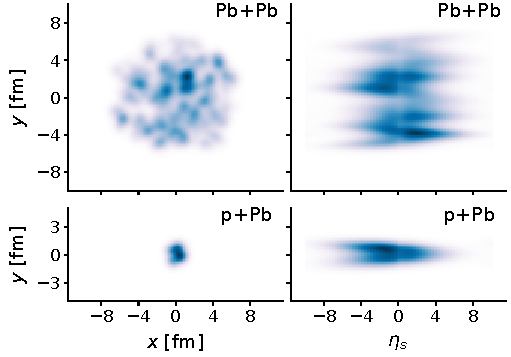
\includegraphics[width=.8\textwidth]{trento3d/trento3d_example}
\caption[Two sample events for Pb-Pb collision (top row) and p+Pb]{Two sample events for Pb-Pb collision (top row) and p+Pb collision (bottom row). The left column and the right column slice the initial entropy density at middle rapidity and the $x=0$ plane respectively. The relative skewness parametrization is used with $\mu_0=1$, $\sigma_0=3$ and $\gamma_r=6$.}
\label{fig:3d-example}
\end{figure}

In figure \ref{fig:3d-example}, we show two sample events from a $Pb$-Pb collision (top plots) and a $p$-Pb collision (bottom plots) generated by \trento\ .
The 3D initial entropy densities are sliced at mid-rapidity $\eta_s=0$ (left plots) and at the $x=0$ plane (right plots).
The mid-rapidity results are identical to the one predicted in the original \trento\ model.
The model is capable of generating fluctuating longitudinal structures that are local in the transverse plane, and breaking the boost-invariance both locally and globally.
For the $p$-Pb event, there is a clear structure that one hot spot extends into the proton going side $\eta_s >0$, while the participant clusters from the lead nuclei push the entropy production into the lead going side $\eta_s <0$.

\section{Reverse engineering the 3D initial condition}
In the final section of this chapter, I apply the hydrodynamic-based simulation framework and the flexible \trento-3D initial condition model to reverse engineer the 3D entropy deposition at the onset of hydrodynamics at LHC energies.

Experimentally, one can only measure rapidity-dependent observables on an event averaged level, which already integrates the contribution of particle production over the transverse plane; while our parametrization in the \trento\ model only involves local functions of the participant density function.
So it is a nontrivial task to infer the functional form of local entropy production $s(\x, \eta_s)$ from these ``global'' measurements.
The statistical technique for the reverse-engineering is the Bayes analysis explained in chapter \ref{chapter:bayes}.

\subsection{Sensitive observables to the initial entropy deposition}
\paragraph{The single particle spectra}
The most direct observable is the charged particle pseudo-rapidity density $\dnchdy$ measured for different collision systems and centralities.
The ALICE collaboration and the ATLAS collaboration has measured this quantity for both the Pb-Pb system ($-3.5<\eta<5.0$) and the p-Pb system ($|\eta| < 2.7$).
$\dnchdy$ can very well constrain the global rapidity profile and the centrality dependence of the mode, while the limitation being that it is less sensitive to the amount of longitudinal fluctuations.

\paragraph{Two particle pseudo-rapidity correlation}
A good probe of event-by-event longitudinal fluctuations is the two-particle pseudorapidity correlation observable $C(\eta_1, \eta_2)$,
\begin{eqnarray}
C(\eta_1, \eta_2) = \frac{ \left\langle N(\eta_1)N(\eta_2) \right\rangle}{\left\langle N(\eta_1)\right\rangle\left\langle N(\eta_2) \right\rangle}
\end{eqnarray}
The long range part of $C(\eta_1, \eta_2)$ is sensitive to the initial state.
This is because the correlation between particles separated by a large rapidity gap at proper time $\tau$ can only come from proper times before $\tau e^{-|\eta_1-\eta_2|/2}$ due to causality.
For example, if two particles separated by four units of rapidity are emitted at a constant $\tau = 8$ fm/$c$ hydrodynamic freeze-out hyper-surface and neglecting the long range correlation from the hadronic cascade, then any correlation must have come from before the proper time $ 8 e^{-2}\approx 1$ fm/c.

To see how $C(\eta_1, \eta_2)$ is related to the longitudinal fluctuation of the entropy deposition / particle production, decompose $\dnchdy$ for each event in a finite pseudo-rapidity window $[-Y, Y]$ using the normalized Legendre polynomials basis \cite{Bzdak:2012tp, Jia:2015jga, ATLAS:2015kla},
\begin{eqnarray}
\frac{dN}{d\eta} &=& \biggl\langle\frac{dN}{d\eta}\biggr\rangle \biggl[1 + \sum_{n=0}^\infty a_n T_n\left(\frac{\eta}{Y}\right) \biggr],\\
T_n(x) &=& \sqrt{n + \frac{1}{2}} P_n(x)
\end{eqnarray}
Where $\langle\frac{dN}{d\eta}\rangle$ is the reference multiplicity at mid-rapidity for a certain centrality.
$a_0$ is the total multiplicity fluctuation and $a_1$ controls how the multiplicity distribution is tilted in rapidity in each event and so on.
The two-particle correlation $C(\eta_1, \eta_2)$ measures the variance of these $a_n$ coefficients.
Define the normalized event-wise distribution $R(\eta) = dN/d\eta /\langle dN/d\eta\rangle$, then the correlator is,
\begin{eqnarray}
C(\eta_1, \eta_2) &=& \left\langle R(\eta_1) R(\eta_2)\right\rangle \\
&=& 1 + \sum_{m, n}\langle a_m a_n\rangle  T_{mn}(\eta_1, \eta_2),\\
T_{mn}(\eta_1, \eta_2) &=& \frac{T_n(\eta_1)T_m(\eta_2) + T_m(\eta_1)T_n(\eta_2)}{2}.
\end{eqnarray}
Therefore, $\langle a_m a_n\rangle$ can be extracted by projecting the two particle correlation on to the function $T_{mn}$.

Combinations like $\langle a_0 a_n\rangle$ simply reflect how the event-wise rapidity fluctuation correlates with the multiplicity fluctuation. 
These contributions are canceled to first order by another normalization to define $C_N$,
\begin{eqnarray}
 C_N(\eta_1, \eta_2) &=& \frac{C(\eta_1, \eta_2)}{C_1(\eta_1)C_2(\eta_2)},\\
C_{1,2}(\eta_{1,2}) &=& \int_{-Y}^{Y}C(\eta_1, \eta_2)\frac{d\eta_{2,1}}{2Y}.
\end{eqnarray}
Finally, $C_N$ is directly related to the rapidity fluctuation itself,
\begin{eqnarray}
C_N(\eta_1, \eta_2) \sim 1 + \frac{3}{2}\langle a_1 ^2 \rangle \frac{\eta_1\eta_2}{Y^2} + \cdots.
\end{eqnarray}
We make use of the $\langle a_1 ^2 \rangle$ measurements to constrain the amount of linearly-tilting fluctuation in the initial condition model.

In additional to the initial condition fluctuation, short range correlation also contribute to the $a_1$ fluctuation \cite{Denicol:2015bnf}.
The UrQMD hadronic afterburner is able to model certain type short range correlations coming from resonance decay and collisions, but jet-like correlations are hard to accounted for.

\subsection{Calibration of the 3D initial condition parameters}
The degrees of freedom of the initial condition model are,
\begin{itemize}[itemsep=0pt]
  \item[1--2.] Two normalization factors for Pb-Pb and p+Pb collisions at $\sqrts=2.76$~TeV and 5.02~TeV beam energies. They are not fully independent as $N_{\textrm{p+Pb}} > N_{\textrm{Pb-Pb}}$ is always imposed in the parameter sweep.
  \item[3.] The mid-rapidity entropy deposition parameter $p$.
  \item[4.] The $\Gamma$-fluctuation variance parameter $1/k$.
  \item[5.] The Gaussian nucleon width $w$, which determines the initial state granularity.
  \item[6--8.] Three coefficients that modulate the local rapidity distribution's shift $\mu_0$, width $\sigma_0$, and skewness $\gamma_r$ or $\gamma_a$,
  \item[9.] An average Jacobian $J$ for the conversion from rapidity to pseudorapidity.
\end{itemize}
The range of the parameters is shown in \ref{tab:trento:parameters}.
One may notice that we did not use different width parameters for the rapidity distribution $\sigma_0$ for Pb-Pb and p-Pb collisions, because the beam rapidity changes less than $8\%$ from $2.76$ TeV to $5.02$ TeV.

\begin{table}
\centering
\caption{Three-dimensional initial condition parameters}
\label{tab:trento:parameters}.
\begin{tabular}{lll}
      Parameter & Description	& Range \\
      \paddedhline
      $N_{\textrm{p+Pb}}$    & Overall p+Pb normalization      & 140.0--190.0 \\
      $N_{\textrm{Pb-Pb}}$   & Overall Pb-Pb normalization     & 150.0--200.0  \\
      $p$	                   & Generalized mean parameter      & -0.3--0.3 (with a prior)  \\
      $k$	                   & Multiplicity fluct.\ shape      & 1.0--5.0  \\
      $w$	                   & Gaussian nucleon width     & 0.4--0.6  \\
      $\mu_0$                & Rapidity shift mean coeff.\     & 0.0--1.0  \\
      $\sigma_0$             & Rapidity width std.\ coeff.\    & 2.0--4.0  \\
      \multirow{2}{*}{$\gamma_0$}             & \multirow{2}{*}{Rapidity skewness coeff.\ }      & 0.0--10.0 (rel) \\
                  &        & 0.0--3.6 (abs)  \\
      $J$	                   & Pseudorapidity Jacobian param.  & 0.6--0.9
\end{tabular}  
\end{table}

The dynamical model consists of a 3+1D relativistic hydrodynamics and a hadronic afterburner.
The equation-of-state (EoS) is obtained by interpolating the state-of-the-art lattice-QCD EoS \cite{Bazavov:2014pvz} at high temperature (zero baryon density) to a hadron resonance gas EoS at low temperature \cite{Moreland:2015dvc}.
The energy density at which the hydrodynamic energy momentum tensor is particulized into hadrons is $\epsilon_{sw} = 0.322$~GeV/fm$^3$ corresponding to a switching temperature close to the pseudo-critical temperature $T_{sw} \sim T_c = 0.154$~GeV).
As a remark, the relativistic hydrodynamics code vHLLE \cite{Karpenko:2013wva} includes viscous corrections, but we used its ideal mode in the parameter extraction.
This is because the parameter optimization process requires running the model on hundreds of different parameter sets.
For each parameter set, thousands of minimum-biased events needed to be generated to control the statistical uncertainty, especially for the correlation observables. 
The full 3+1D viscous hydrodynamics is extremely time consuming, therefore we choose to run the hydrodynamic model in its ideal mode and on a rather coarse grid.
The justification is that the rapidity distribution of the multiplicity and normalized two-particle correlations is less sensitive to the viscosity.
In the end, as a validation of this procedure, we will be using a set of high-likelihood parameters and run the dynamical model with the viscous mode of the hydrodynamic model to see if other observables such as the anisotropic flows, and event-plane decorrelations can be described.

\begin{figure}
\singlespacing 
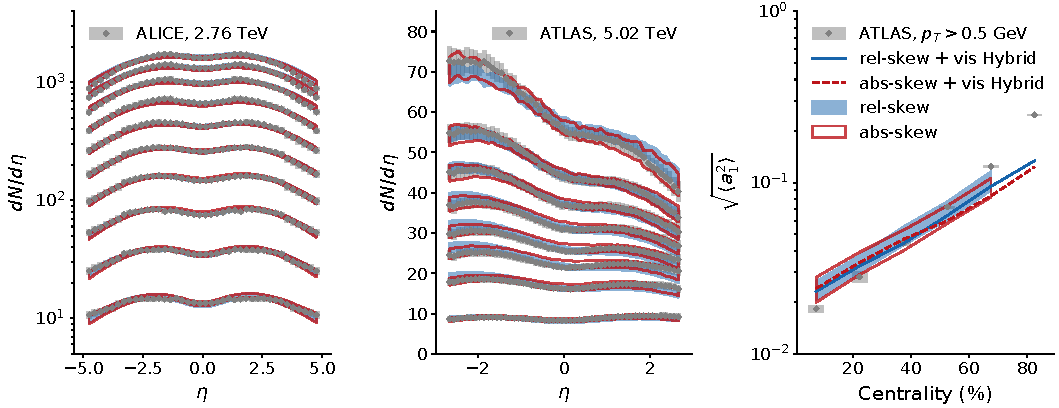
\includegraphics[width=\textwidth]{trento3d/post_obs.pdf}
\caption[The posterior distribution of the observables after the fitting]{The posterior distribution of the observables after the fitting process. Blue and red stands for the results calibrated using the ``relative skewness'' and the ``absolute skewness'' ansatz respectively.
From left to the right are charged particle pseudorapidity density in Pb-Pb collision, in p+Pb collision, and the rms of the $a_1$ coefficient in the two-particle pseudorapidity correlation decomposition. The lines in the right most figure shows that the rms $a_1$ is not very sensitive to the viscous effect in the hydrodynamic evolution.}
\label{fig:trento:post_obs}
\end{figure}

Four thousands Pb-Pb and ten thousands p-Pb events are generated at $100$ sets of parameter values, then the Bayesian analysis makes inference on the probability distribution of the parameters by comparing to measurements.
After the calibration, the $\dnchdy$ and $a_1$ fluctuations as function of centrality are compared to measurements in figure \ref{fig:trento:post_obs}.
The single particle distribution can be well reproduced by the calibrated initial condition plus dynamical evolution, while the correlation observables can be described up to 50\% centrality. 
For more peripheral Pb-Pb collisions, the hydrodynamic model significantly underestimate the $a_1$ fluctuation.
We understand this as a consequence of inadequate modeling of the short range correlation for peripheral collisions, as they are more important in low multiplicity events ($\dnchdy\sim 250$ and $N_{\textrm{part}} \sim 75$ at 50\% centrality).
In fact, the authors of \cite{ATLAS:2015kla} compared the measurements to the HIJING event generator that is based on mini-jet production.
It is found that these jet-like correlations agrees well with the $a_1$ fluctuation for peripheral collisions with $N_{\textrm{part}} \lesssim 80$, while it overshoots the data for more central collision.
The hydrodynamic model and mini-jet production model provide a complementary picture to fully understand the rms $a_1$: at larger centrality, mini-jet production dominates the fluctuation of the $\dnchdy$, while as multiplicity increases and the final state interactions are frequent, the event-by-event asymmetry in the single-particle distribution dominates the rms $a_1$.

\begin{figure}
\singlespacing 
\centering
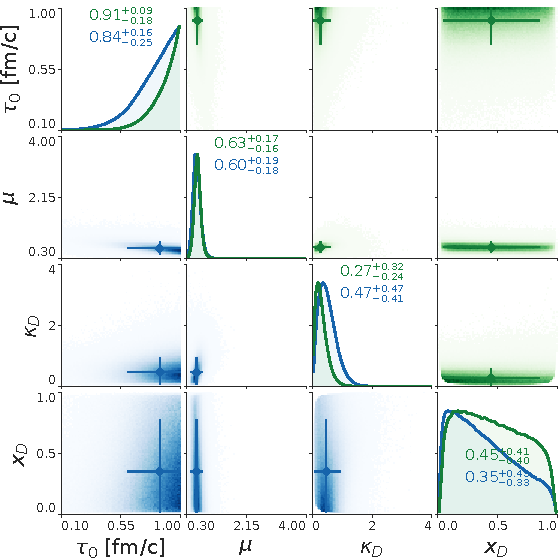
\includegraphics[width=\textwidth]{trento3d/posterior.pdf}
\caption[The posterior probability distribution of the model parameters,]{The posterior probability distribution of the model parameters, the colors distinguish the use of ``absolute skewness'' (red) and ``relative skewness'' ansatz. The diagonals are single parameter distribution, the off-diagonals are two-parameter joint distributions.}
\label{fig:trento:posterior}
\end{figure}

Regarding the performance of different parametrizations of the skewness, the ``relative'' skewness ansatz does better in reproducing the uprising trend of rms $a_1$, while the absolute skewness ansatz better describes the large $\dnchdy$ asymmetry in the top 1\% p+Pb collisions.
However, there is no strong evidence to favor any of them over the other.
We will see later that this is because the two parametrizations, though take different forms, actually behave similar in terms of $ds/d\eta(\eta; T_A, T_B)$, for typical values of $T_A$ and $T_B$ of heavy nuclei.

\begin{figure}
\singlespacing 
\centering
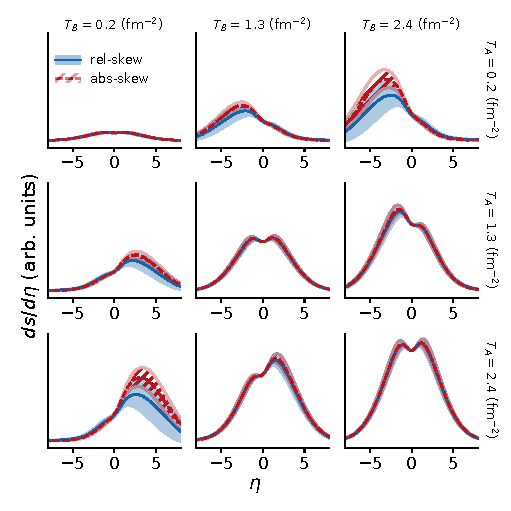
\includegraphics[width=.8\textwidth]{trento3d/post_dsdy}
\caption[The constrained functional form of the three-dimensional initial]{The constrained functional form of the three-dimensional initial entropy deposition $s(T_A(\mathbf{x}_\perp), T_B(\mathbf{x}_\perp), \eta_s)$. $T_A$ and $T_B$ is varied from $0.2$ to $2.4$ fm${}^{-2}$. Colors distinguish the results from using ``absolute skewness'' (red) and ``relative skewness'' ansatz.}
\label{fig:trento:post_dsdy}
\end{figure}

The distribution of the calibrated parameters is shown in figure \ref{fig:trento:posterior}.
The red and blue lines and color map correspond to results using the ``absolute'' and ``relative'' skewness respectively.
The normalization parameters $N_{\textrm{PbPb}}$ and $N_{\textrm{pPb}}$, mid-rapidity entropy deposition parameter $p$, nucleon thickness function fluctuation parameter $k$, the width of the rapidity distribution $\sigma_0$ and the effective Jacobian $J$ have similar probability distributions between the two parametrizations.
However, the distribution of the asymmetry related parameters $\mu_0$ and $\gamma_0$ (anti-correlated), and nucleon width $w$ are very different.
This is because the Bayesian calibration looks for the high-likelihood region of the parameter space to explain the data, and the two different prarametrizations can achieve this same goal by optimizing the parameter combinations differently.
For the ``relative'' skewness one, the optimized parameters have a small shift of the mean $\mu$ and a large skewness $\gamma$; for the ``absolute'' skewness one, they correspond to the region with a large $\mu$ but vanishing $\gamma$.
This does not mean that there are ``two models'' explaining the same data, because both of them are an oversimplified parametrization of $ds/d\eta(\eta; T_A, T_B)$ with infinitely many degrees of freedom. 
Instead, we should treat them as an estimation of the systematic uncertainty in extracting the function form of the initial 3D entropy deposition $ds/d\eta(\eta; T_A(\x), T_B(\x))$.
It is more instructive to see the probability distribution of $ds/d\eta$ it self, given different values of $T_A(\x)$ and $T_B(\x)$.
In Fig.~\ref{fig:trento:post_dsdy}, we samples the calibrated parameter distributions and use them to draw the entropy density as function of rapidity at different values of $T_A$ and $T_B$. 
Again, the red and blue colors represents ``absolute'' and ``relative'' skewness parametrizations; the lines shows the median prediction and the bands are one standard deviation uncertainties. 
In each row and each column, $T_A$ and $T_B$ varies from $0.2~\text{fm}^{-2}$ to $2.4~\text{fm}^{-2}$. 
For references, the value of the thickness function at the center of a Gaussian proton with nucleon width $0.5$ fm is about $0.6~\text{fm}^{-2}$ and is $0.2~\text{fm}^{-2}$  at 1.5 width away from its center; while the maximum nuclear thickness function of a Pb nucleus is about $2.2~\text{fm}^{-2}$.
Therefore, the chosen range of $T_{A,B}$ already cover the typical ranges and combinations for entropy production in a realistic heavy-ion collision.
One observe that the functional form of the $ds/dy$ between the two parametrization agrees within one standard deviation, with the deviations increasing as the asymmetry increases.
Certainly, with sufficiently different $T_A$ and $T_B$ combinations, the two results will have totally different predictions; however, within the physical range of the thickness function, the two methods converges onto a similar behavior,
We conclude that by applying the hydrodynamic-based model and a flexible 3D initial condition, the form of the local rapidity distribution as function of participant densities can be reverse engineered using single particle pseudo-rapidity distributions and two-particle pseudo-rapidity correlations.

\subsection{Prediction with the calibrated 3D initial condition}
The calibrated initial condition is useful in predicting other rapidity-dependent observables.
Especially, because we have only used multiplicity based observables $\dnchdy$ and rms $a_1$ in the calibration, a prediction of azimuthal anisotropy related observables would provide an important validation of the initial condition.
We choose a set of high-likelihood parameters shown in table \ref{tab:chosen_parameters}.
The selected validation / prediction observables are pseudo-rapidity dependent harmonic flows, event-plane decorrelations and the symmetric cumulants which quantify the correlation between different flow harmonics.

\begin{table}
\centering
\caption{A high likelihood parameter set}
\begin{tabular}{lll}
\hline
Parameter & rel-skew	& abs-skew \\
\hline
$N_{\textrm{Pb-Pb}}$   & 150.0     & 154.0  \\
$p$	    & 0.0      & 0.0  \\
$k$	    & 2.0     & 2.0  \\
$w$	    & 0.59     & 0.42  \\
$\mu_0$   & 0.0     & 0.75  \\
$\sigma_0$ & 2.9    & 2.9  \\
$\gamma_0$ & 7.3		& 1.0	\\
$J$	     & 0.75 & 0.75	\\
\hline
\end{tabular}
\label{tab:chosen_parameters}    
\end{table}

\paragraph{Mid-rapidity $v_n$} The elliptic and triangular flow from two-particle correlation $v_2\{2\}$ and $v_3\{2\}$ are calculated at as function of centrality at mid-rapidity (figure \ref{fig:trento:vn_cen}) and as function of pesudo-rapidity at different centrality (figure \ref{fig:trento:vn_eta}).
We are able to describe flow measured by ALICE \cite{Adam:2016izf} at mid-rapidity with a shear viscosity $\eta/s = 0.17$--$0.19$ close to other phenomenological studies, though the bulk viscosity is not included in this study.

\begin{figure}
\singlespacing 
\centering
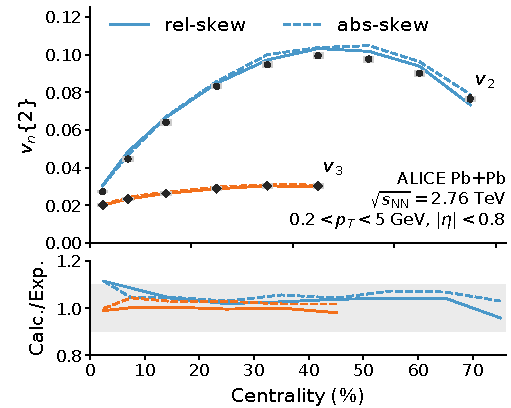
\includegraphics[width=.7\textwidth]{trento3d/vn_cen}
\caption[Flow coefficients $v_2\{2\}$ (blue) and $v_3\{2\}$ (orange) are plotted as]{Flow coefficients $v_2\{2\}$ (blue) and $v_3\{2\}$ (orange) are plotted as a function of centrality. The calculation uses a 3+1D viscous hydrodynamic-based model with constant $\eta/s=0.17$ and $0.19$ for ``relative skewness'' (solid) and ``absolute skewness'' (dashed) ansatz. $\zeta/s=0$ and the switching temperature is $T_\text{sw}=154$~MeV.
The initial condition parameters are selected from the high-likelihood region of the posterior.}
\label{fig:trento:vn_cen}
\end{figure}

\paragraph{Rapidity-dependent $v_n$} For the rapidity dependent flow figure \ref{fig:trento:vn_eta}, we used a larger $\eta/s=0.25$--$0.28$. 
This inconsistency is because the ALICE measurement extrapolates the $p_T$ range for the rapidity-dependent flow down to 0, while the mid-rapidity  $p_T$ cut is $0.2 < p_T < 5.0$ GeV.
It would not be a problem for the model to describe both with the same transport parameters, if the $p_T$ differential flow and $p_T$ differential particle spectra are both reproduced.
However, due to the lack of a systematic tuning of the model parameters including both shear and bulk viscosity, the current mean $p_T$ is too high.
Therefore, agreement with the $p_T$-integrated flow in one kinematic cut does not guarantee the agreement to measurements that extrapolate to $p_T = 0$.
Since our primary interest is the $\eta$-dependence of the flow, we have chosen this larger-than-usual shear viscosity to match the $v_2\{2\}(\eta=0)$ values to data.
The calculated $v_2\{2\}$, $v_3\{2\}$, and $v_2\{4\}$ gradually decrease from mid-rapidity to forward / backward rapidity, which is also the trend seen in the data.
The shape of $v_3\{2\}$ is well described; but for $v_2\{2\}$ and $v_2\{4\}$ in the region $|\eta| > 2.0$, the data decreases faster than our predictions.
There could be several reasons for this difference.
It is possible that the current initial condition model produce enough fluctuations, but inadequate variance of the overlapping geometry as function of space-time rapidity.
It is also showed in a study of at RHIC energies that the decreasing slope of $v_n(\eta)$ can be sensitive to the shear viscosity in the hadronic phase \cite{Denicol:2015bnf, Bozek:2010bi}.
In our model, the transport properties of the system below $T_c$ is all encoded in UrQMD and are not tunable. 
Moreover, we have assumed that hydrodynamization happens at a constant proper time hypersurface;
while it is possible that a constant entropy density hypersurface is a better criteria, and as a result the matter at larger rapidity experiences a shorter period of pressure driven expansion.
To systematically investigate all these effects, a future global parameter calibration including both initial condition parameters, transport parameters, and matching parameters is inevitable and is also feasible given the advances in the dynamical models and programming developments as well as more powerful computing resources.

\begin{figure}
\singlespacing 
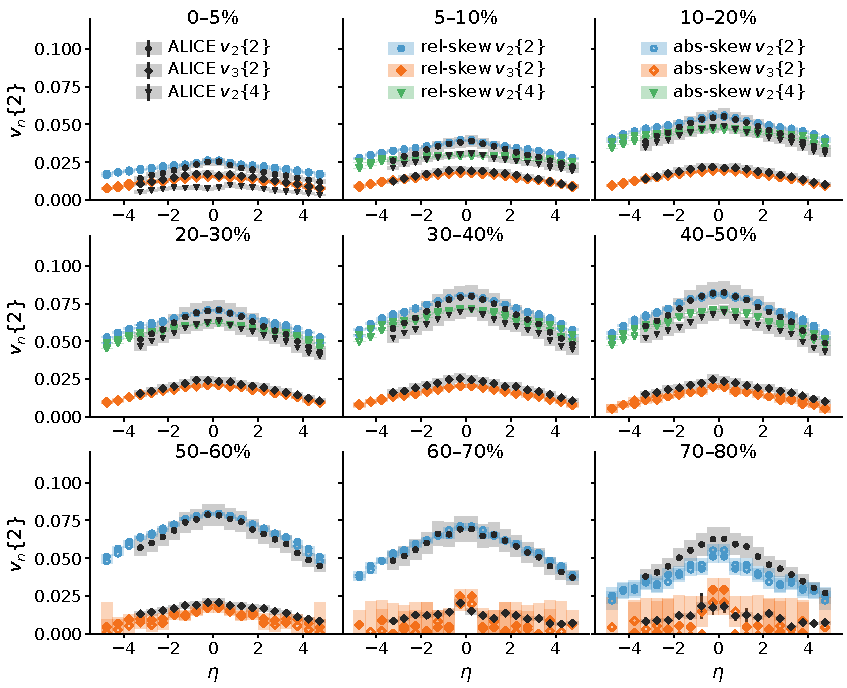
\includegraphics[width=\textwidth]{trento3d/vn_eta}
\caption[Pseudorapidity dependent flow coefficients $v_2\{2\}$ (blue circle), ]{Pseudorapidity dependent flow coefficients $v_2\{2\}$ (blue circle), $v_3\{2\}$ (green triangle) and $v_2\{4\}$ (orange diamond).
Constant $\eta/s=0.25$ and $0.28$ are used for ``relative skewness'' (closed symbol) and ``absolute skewness'' (open symbol) ansatz. Data is taken from the ALICE Collaboration \cite{Adam:2016ows}.}
\label{fig:trento:vn_eta}
\end{figure}

\paragraph{Event-plane decorrelations} The event-planes are defined as the phase angle of the anisotropic flow,
\begin{eqnarray}
\Psi_n^\text{EP} = \frac{\text{atan2}(\langle \sin n \phi \rangle, \langle\cos n \phi \rangle)}{n},
\end{eqnarray}
Due to longitudinal fluctuations, the event-planes separated by a rapidity gap decorrelate from each other.
This decorrelation is important for observables that involve a large rapidity gap.

This event-plane decorrelation has been studied using initial conditions from a 3D extended Glauber model \cite{Bozek:2015bna} and A Multi-Phase Transport (AMPT) model \cite{Jia:2014ysa, Xiao:2012uw,Pang:2015zrq}.
Gluonic Yang-Mills dynamics in three-dimensions have also been used to study decorrelation at the initial stage level \cite{Schenke:2016ksl}.
In our model, the geometry at forward and backward rapidity are dominated by the participant density of two different nuclei.
And in between, the entropy production smoothly transit from one to anther and so are the orientation of the energy density eccentricities that drive the flow of particles.
The CMS collaborations quantifies the decorrelation by a three-bins factorization ratio \cite{Khachatryan:2015oea},
\begin{eqnarray}
r_n(\eta^a, \eta^b) &= \frac{V_{n\Delta}(-\eta^a, \eta^b)}{V_{n\Delta}(\eta^a, \eta^b)}, \\
V_{n\Delta}(\eta^a, \eta^b) &= \langle\langle \cos(n\Delta\phi) \rangle\rangle,
\end{eqnarray}
where the double average runs over all particle pairs and all events.
One of the rapidity bins is near $\eta^b$ and the rest of the two bins are around $\pm\eta^a$.
This ratio measures the decorrelation between two event planes separated by a larger rapidity gap $\eta^a + \eta^b$ relative to the decorrelation over a smaller gap $|\eta^a - \eta^b|$.
In experiments, one would like to take the reference bin $\eta^b$ farther from $\eta_a$ to suppress the short range correlations correlation.
However, the way we build our model is to extend the mid-rapidity entropy deposition to finite rapidity, and this extension will eventually fail at sufficiently large rapidity because the model behavior in those region is not well constrained.
In figure \ref{fig:trento:epd}, we compare the model calculations to data with both a large $4.4<\eta^b<5.0$ (bottom) and a relative smaller $3.0 < \eta^b< 4.0$ (top).
The predicted factoziation ratios decreases linearly with the increasing rapidity gap.
Using reference particles from $3.0 < \eta^b< 4.0$, the decorrelation is reproduced at larger centrality but not for central collisions.
Because the $n=2$ event-plane has a preferred direction defined by the impact parameter, while $n=3$ event-plane does not, we observe that the $n=2$ factorization ratio decorrelates slower than the $n=3$ ratio, except for the most central collision when $n=2$ event-plane is also dominated by fluctuations.
Comparing to data with reference particles from $4.4<\eta^b<5.0$, the experimental data stays similar to the the previous case except for central collisions, but the prediction is completely off.
This is simply because the model fails on the details at large rapidity as we explained earlier.
Given the present comparison, we conclude that the valid range of the model should be restricted to $|\eta| < 4.0$.

\begin{figure}
\singlespacing 
\centering
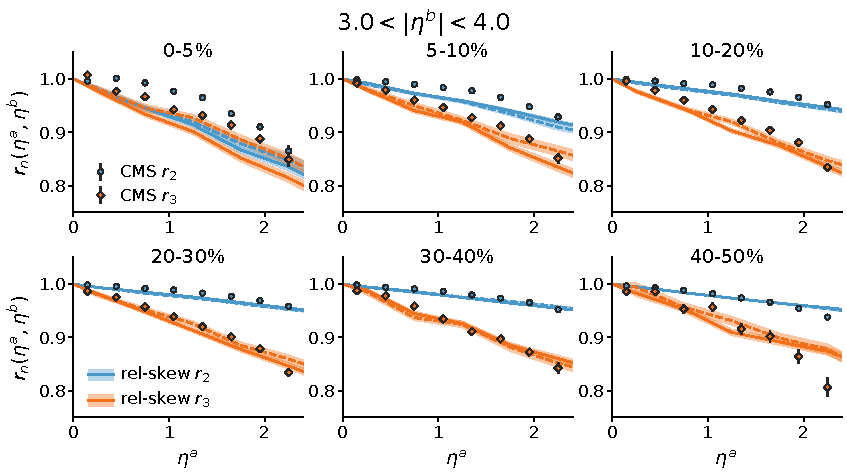
\includegraphics[width=.8\textwidth]{trento3d/evt_pln_decorr_near}\\
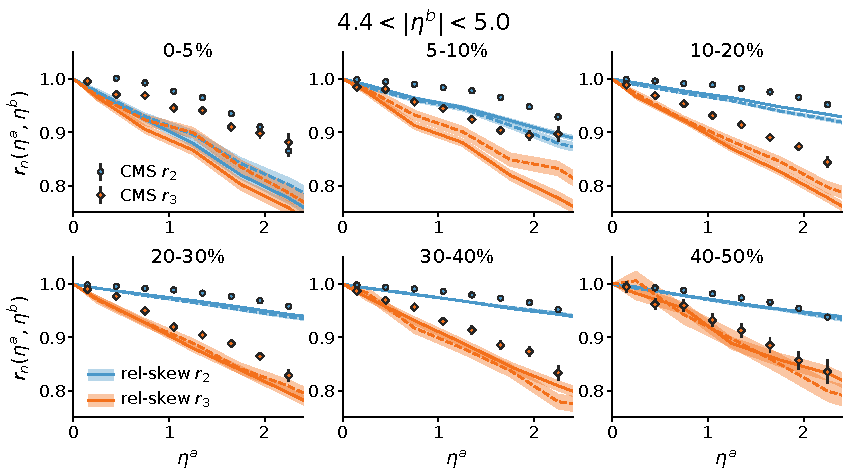
\includegraphics[width=.8\textwidth]{trento3d/evt_pln_decorr_far}
\caption[The $n=2$ (blue) and $n=3$ (orange) event-plane decorrelations]{The $n=2$ (blue) and $n=3$ (orange) event-plane decorrelations obtained for ``relative skewness'' (lines with bands) and ``absolute skewness'' (lines with hatches) ansatz. The top and bottom plots uses different reference particle bins $3.0<|\eta_b|<4.0$ and $4.4<|\eta_b|<5.0$ respectively.}
\label{fig:trento:epd}
\end{figure}

\paragraph{Symmetric cumulants} Finally, we predict the symmetric cumulants (SC), which is a four particle correlation between different orders of anisotropic flows $v_m$ and $v_n$ \cite{Niemi:2012aj,Bilandzic:2013kga}.
\begin{eqnarray}
SC(m, n) &=& \langle\langle \cos(m\phi_1+n\phi_2-m\phi_3-n\phi_4)\rangle\rangle \nonumber \\
\nonumber &-& \langle\langle\cos[m(\phi_1-\phi_2)]\rangle\rangle\langle\langle\cos[n(\phi_1-\phi_2)]\rangle\rangle \label{eq:scmn}\\
&=& \langle v_m^2 v_n^2 \rangle - \langle v_m^2\rangle\langle v_n^2\rangle.
\end{eqnarray}
It is clear from the second equation that it measures the covariance between $v_n^2$ and $v_m^2$.
One can also define the normalized symmetric cumulants (NSC),
\begin{equation}
NSC(m,n) = \frac{SC(m,n)}{\langle v_m^2\rangle\langle v_n^2\rangle}.
\end{equation}
These observables are interesting because they are robust against non-flow effects, and have been shown to be sensitive to the temperature dependece of the transport coefficients \cite{ALICE:2016kpq}.
Other analysis show that $SC(4,2)$ probes the non-linear response of the hydrodynamic evolution, while $SC(3,2)$ is more sensitive to initial conditions \cite{Zhu:2016puf}.



The relative- and absolute-skewness calculations are arranged on the left and right of \ref{fig:trento:smn}. 
Symmetric cumulants $SC(4,2)$ (blue) and $SC(3,2)$ (green) are displayed in the top plots, and $NSC(4,2)$ (blue) and $NSC(3,2)$ (green) in the bottom plots.
Within each plot, black dots are ALICE measurements at midrapidity $|\eta|<0.8$ \cite{ALICE:2016kpq}, which should be compared to the calculation shown in solid lines.
The calculation shown in dashed lines are our predictions at forward/backward rapidity $2.5 < |\eta| < 3.5$,
\begin{eqnarray}
SC^\prime(m, n) &=& \langle\langle \cos(m\phi_1+n\phi_2-m\phi_3^\prime-n\phi_4^\prime)\rangle\rangle \\
\nonumber &-& \langle\langle\cos[m(\phi_1-\phi_2^\prime)]\rangle\rangle\langle\langle\cos[n(\phi_1-\phi_2^\prime)]\rangle\rangle, \label{eq:scmn-diff}
\end{eqnarray}
where the two of the particles (primed) are selected from the forward/backward rapidity bins, while the rest of the two still come from the mid-rapidity bin $|\eta|<0.8$.

At mid-rapidity, the calculated (normalized) symmetric cumulents reproduce the trend of the measurements, and the ``relative'' skewed initial condition does a better quantitative job than the ``absolute'' skewed model.
At forward and backward rapidity, though the magnitudes of both $SC(m,n)$ and $v_n$, $v_m$ changed, the normalized symmetric cumulants remains the same as the one at mid-rapidity.
This is a prediction that can be checked in future measurements to put further constraints on the three-dimensional initial condition model.

\begin{figure}
\singlespacing 
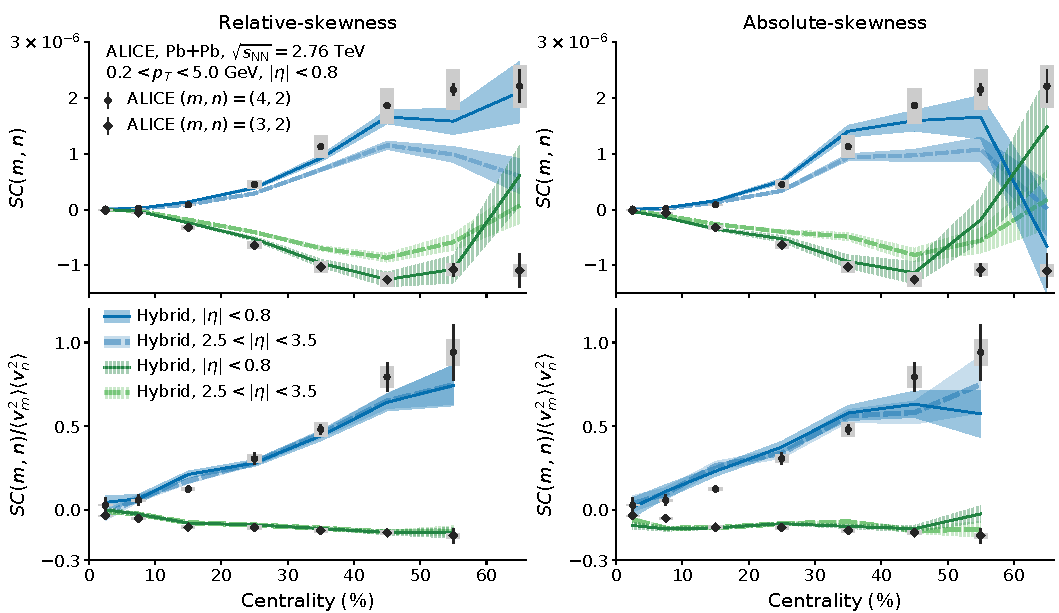
\includegraphics[width=\textwidth]{trento3d/smn}
\caption[The symmetric cumulants (top row) and normalized symmetric]{The symmetric cumulants (top row) and normalized symmetric cumultants (bottom row) obtained from the ``relative skewness'' (left column) and the ``absolute skewness'' (right column) ansatz.
$SC(4,2)$ (blue) and $SC(3,2)$ (green) are shown as functions of centrality. The experimental measurements at mid-rapidity (black symbols) are taken from \cite{ALICE:2016kpq}.
The calculations are performed at both mid-rapidity $|\eta|<0.8$ (solid lines) and forward/backward rapidity $2.5<|\eta|<3.5$ (dashed lines).
}
\label{fig:trento:smn} 
\end{figure}

As a summary of this chapter, I have introduced the hydrodynamic-based  medium evolution model that is very successful in describing the bulk observables.
The sensitivity of the harmonic flows allows one to extract QCD transport coefficients using advanced statistical techniques.
The initial condition for the dynamical model is still a large source of uncertainty in both data interpretation and parameter extraction.
The \trento\ model was developed as a flexible ansatz for mid-rapidity entropy / energy deposition so that the initial condition and transport coefficients can be calibrated simultaneously to data.
Finally, I discussed my work on extending the \trento\ initial condition to include rapidity dependence and the use of multiplicity observable to reverse-engineer the functional form of initial 3D entropy deposition.
The results can be used to predict more rapidity-dependent observables, and are useful to other studies involving a large rapidity range.
Due to the simplicity of the modeling, and the lack of global fit of all parameters including both 3D initial conditions and transport coefficients, we cannot yet answer how the inclusion of longitudinal fluctuation quantitatively affects the extracted QCD transport coefficients, but it is an important question for a future precision analysis.